\section{Sign reversal and the decomposition}
\label{sec:negative}
\paragraph{Why flip rates cannot be compared across strata.}
A memory can show a flip only if at least two of its cells move with opposite
signs, so the chance of a flip grows with the number of cells per memory. In
the screened design a memory has $\raCellsPerMemBear$ \textsc{bearing} cells
and $\raCellsPerMemRand$ \textsc{random} cells on average. The naive
contrast (0 of 35 \textsc{bearing} memories against 17 of 60 \textsc{random},
Fisher one-sided $p = 1.5\times10^{-4}$) therefore mostly reflects that
difference. To test this, we took each of the $\raMatchedN$ memories with at
least two \textsc{bearing} cells and drew, without replacement, as many of its
\textsc{random} cells as it has \textsc{bearing} cells, then recounted flips
(20{,}000 resamples). The random stratum averages $\raMatchedMean$ flips and
shows none in $\raMatchedPZero\%$ of resamples (Figure~\ref{fig:reversal}b), so
0 of 35 is what chance alone would most often produce. A Wilson bound on the \textsc{bearing} flip rate would also treat 35 memories
from 21 episodes as independent.
Matching each memory's random subsample on the no-memory outcome as well (so
both strata get the same opportunities to help and to hurt) leaves all
$\lfCondFlipMems$ memories eligible; the random stratum then shows a mean of
$\lfCondFlipMean$ flips and none in $\lfCondFlipPZero\%$ of resamples. We
therefore do not compare flip rates across strata.

\paragraph{Why the sign of moving cells is not a comparison either.}
A tempting alternative compares the share of negative cells among cells that
move: $\raNegBearK$ of $\raNegBearN$ for \textsc{bearing} against
$\raNegRandK$ of $\raNegRandN$ for \textsc{random}. That comparison is
confounded by baseline accuracy. A memory can only hurt where the reader was
correct without it, and \textsc{bearing} tasks have the lowest no-memory
accuracy, so they offer the fewest chances to hurt.

\paragraph{Transitions conditioned on the no-memory outcome.}
Reward is binary in the screened run: each stratum's mean equals
(helped $-$ hurt)$/n$ exactly. With Table~\ref*{M-tab:screened}'s both-arms-fail
rate this fixes the full transition table (Table~\ref{tab:transitions}).
Conditioned on opportunity, the strata do not differ detectably in harm,
and they differ sharply in help (Figure~\ref{fig:reversal}a). In the
\textsc{random} stratum help and harm rates are close, the signature of a
content-independent response to inserting an item, which we treat as the
perturbation floor (\main{sec:metrics}). The table's Wilson intervals treat cells as
independent. Resampling memories instead, the harm rates have intervals of
$[\lfHurtClBearLo, \lfHurtClBearHi]$ (\textsc{bearing}),
$[\lfHurtClCtrlLo, \lfHurtClCtrlHi]$ (control) and
$[\lfHurtClRandLo, \lfHurtClRandHi]$ (\textsc{random}), which overlap, and the
help rates $[\lfHelpClBearLo, \lfHelpClBearHi]$,
$[\lfHelpClCtrlLo, \lfHelpClCtrlHi]$ and $[\lfHelpClRandLo, \lfHelpClRandHi]$,
where \textsc{bearing}'s is disjoint from the others. Both
analyses here are exploratory and are produced by
\texttt{make\_reanalysis.py}, which first checks that it reproduces every flip
count and stratum mean in the paper.

\begin{table}[t]
\centering\footnotesize
\setlength{\tabcolsep}{2.6pt}
\caption{Screened run on LongMemEval-V2: transitions between the no-memory
and with-memory outcome (binary reward). Accuracy columns give the share of
cells answered correctly without and with the memory. Hurt is conditioned on
cells correct without the memory, help on cells wrong without it; Wilson 95\%
intervals in brackets.}
\label{tab:transitions}
\begin{tabular}{@{}lrrrrr@{}}
\toprule
stratum & $n$ & acc.\ w/o & acc.\ with & hurt $\mid$ correct & help $\mid$ wrong \\
\midrule
\textsc{bearing} & \spBearN & \raAccZeroBear & \raAccOneBear
  & \raHurtRateBear\ [\raHurtLoBear, \raHurtHiBear] & \raHelpRateBear\ [\raHelpLoBear, \raHelpHiBear] \\
control & \spCtrlN & \raAccZeroCtrl & \raAccOneCtrl
  & \raHurtRateCtrl\ [\raHurtLoCtrl, \raHurtHiCtrl] & \raHelpRateCtrl\ [\raHelpLoCtrl, \raHelpHiCtrl] \\
\textsc{random} & \spRandN & \raAccZeroRand & \raAccOneRand
  & \raHurtRateRand\ [\raHurtLoRand, \raHurtHiRand] & \raHelpRateRand\ [\raHelpLoRand, \raHelpHiRand] \\
\midrule
\multicolumn{6}{@{}l}{\emph{opportunities:} hurt $\raHurtOppBear$ / $\raHurtOppCtrl$ / $\raHurtOppRand$ cells;
help $\raHelpOppBear$ / $\raHelpOppCtrl$ / $\raHelpOppRand$ cells} \\
\bottomrule
\end{tabular}
\end{table}

\paragraph{The additive-null comparison.}
Fitting $\mu + a_m + b_t$ and simulating from it, the excess of the observed
reversal rate over the fitted additive model is negative in all three strata.
Two independent implementations agree on the sign and disagree on the
magnitude, so we quote only the sign.

\paragraph{Why the decomposition is not identifiable.}
The within-session execution floor is exactly zero: replicates issued 0--16
seconds apart agree on 1{,}157 of 1{,}157 cells. With no residual scale, the
fitted residual collapses and the task and interaction shares are not
separately identified, so we report none. Clean per-cell utilities and a
variance decomposition are in tension on a reader without execution noise.

\begin{figure}[t]
\centering
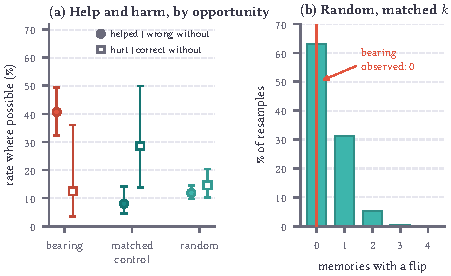
\includegraphics[width=\columnwidth]{fig_reversal}
\caption{Sign reversal on LongMemEval-V2, screened design (1{,}157 cells,
60 memories). \textbf{(a)}~Help rate among cells the reader got wrong without
the memory (filled) and harm rate among cells it got right (hollow), with
Wilson 95\% intervals; counts are in Table~\ref{tab:transitions}. Harm does not differ detectably across
strata; help does. \textbf{(b)}~Flips among the 35 memories with at least two
\textsc{bearing} cells when each memory's \textsc{random} cells are subsampled
to its own \textsc{bearing}-cell count (20{,}000 resamples); the line marks the
observed \textsc{bearing} count.}
\label{fig:reversal}
\Description{Left: dot plot of help and harm rates by stratum; help is about 41 percent for bearing against 8 and 12 percent elsewhere, harm overlaps across strata at 12 to 29 percent with wide intervals. Right: histogram of flip counts at matched cell counts, with zero flips in about 63 percent of resamples.}
\end{figure}
